\documentclass{cstd}

\usepackage{amsmath}
\usepackage{amssymb}
\usepackage{tikz}
\usepackage{algorithm}
\usepackage{algpseudocode}

\university{St. Francis Xavier University}
\department{Department of Computer Science}
\course{CSCI-531 - Reinforcement Learning}
\courseshort{CSCI-531}
\exam{Temporal Difference Learning}
\examdate{Fall 2025}

\begin{document}

\maketitle

% \printanswers


\begin{questions}

% =====================================================
% PART I: TD FUNDAMENTALS
% =====================================================

\section*{Part I: TD Fundamentals}

\question \textbf{TD Update Rule Derivation}

\begin{parts}
\part Starting from the value function definition $V(s) = \mathbb{E}[G_t | S_t = s]$, show how the TD target $r_{t+1} + \gamma V(s_{t+1})$ is derived.

\begin{solution}
Starting with the definition:
\begin{align}
V(s) &= \mathbb{E}[G_t | S_t = s]\\
&= \mathbb{E}[R_{t+1} + \gamma G_{t+1} | S_t = s]\\
&= \mathbb{E}[R_{t+1} | S_t = s] + \gamma \mathbb{E}[G_{t+1} | S_t = s]\\
&= \mathbb{E}[R_{t+1} | S_t = s] + \gamma \mathbb{E}[V(S_{t+1}) | S_t = s]
\end{align}

The TD target $r_{t+1} + \gamma V(s_{t+1})$ is a sample estimate of this expectation, where:
\begin{itemize}
\item $r_{t+1}$ is a sample of $R_{t+1}$
\item $V(s_{t+1})$ is our current estimate of the value at the next state
\end{itemize}
\end{solution}

\part Write the complete TD(0) update equation and explain each component.

\begin{solution}
\begin{equation}
V(s_t) \leftarrow V(s_t) + \alpha[r_{t+1} + \gamma V(s_{t+1}) - V(s_t)]
\end{equation}

Components:
\begin{itemize}
\item $\alpha \in [0,1]$: Learning rate (how much to update)
\item $r_{t+1} + \gamma V(s_{t+1})$: TD target (new evidence)
\item $r_{t+1} + \gamma V(s_{t+1}) - V(s_t)$: TD error (prediction error)
\item The update moves the estimate toward the target proportional to the error
\end{itemize}
\end{solution}

\part Explain why TD learning is called "bootstrapping" and compare it to Monte Carlo.

\begin{solution}
\textbf{Bootstrapping:} TD learning uses its own estimates to update its estimates (like "pulling yourself up by your bootstraps"). The TD target $r_{t+1} + \gamma V(s_{t+1})$ uses the current estimate $V(s_{t+1})$ rather than waiting for the true return.

\textbf{Comparison to Monte Carlo:}
\begin{itemize}
\item \textbf{Monte Carlo}: Uses actual return $G_t$ - no bootstrapping
\item \textbf{TD Learning}: Uses estimated return $r_{t+1} + \gamma V(s_{t+1})$ - bootstrapping
\item TD can learn from incomplete episodes, MC cannot
\item TD has lower variance but higher bias than MC
\end{itemize}
\end{solution}

\end{parts}

\question \textbf{TD Error Analysis}

Consider a simple 2-state chain: Start → Goal, where the agent receives a reward of +5 when reaching the Goal. $\gamma = 0.9$ and $\alpha = 0.1$.

Current value estimates: $V(\text{Start}) = 3.0$, $V(\text{Goal}) = 0$ (terminal)

\begin{parts}
\part Calculate the TD error when transitioning from Start to Goal.

\begin{solution}
TD error: $\delta_t = r_{t+1} + \gamma V(s_{t+1}) - V(s_t)$

$\delta_t = 5 + 0.9 \times 0 - 3.0 = 5 - 3.0 = 2.0$

The TD error is +2.0, indicating our estimate for Start was too low.
\end{solution}

\part What will be the new value estimate for the Start state after this update?

\begin{solution}
New value: $V(\text{Start}) = V(\text{Start}) + \alpha \times \delta_t$

$V(\text{Start}) = 3.0 + 0.1 \times 2.0 = 3.0 + 0.2 = 3.2$
\end{solution}

\part After many episodes, what should $V(\text{Start})$ converge to and why?

\begin{solution}
$V(\text{Start})$ should converge to $5 \times 0.9^0 = 5.0$.

This is because from Start, the agent always transitions to Goal (terminal) with reward +5, and there are no future states to consider. The expected return is exactly the immediate reward of +5.

If there were a discount factor, it would be $5 \times \gamma^{\text{steps to goal}}$, but since Goal is reached in 1 step: $5 \times 0.9^0 = 5$.
\end{solution}

\end{parts}

% =====================================================
% PART II: TD PREDICTION ALGORITHMS
% =====================================================

\section*{Part II: TD Prediction Algorithms}

\question \textbf{TD(0) Algorithm Implementation}

Consider a 3-state Markov chain with states $A \rightarrow B \rightarrow C$ (terminal).
\begin{itemize}
\item Transition $A \rightarrow B$ gives reward $r = 2$
\item Transition $B \rightarrow C$ gives reward $r = 8$
\item $\gamma = 0.8$, $\alpha = 0.5$
\item Initial estimates: $V(A) = 0$, $V(B) = 0$, $V(C) = 0$
\end{itemize}

\begin{parts}
\part Trace through the first episode $(A \rightarrow B \rightarrow C)$ showing all TD updates.

\begin{solution}
\textbf{Step 1: $A \rightarrow B$ (reward = 2)}
\begin{align}
V(A) &\leftarrow V(A) + \alpha[r + \gamma V(B) - V(A)]\\
&\leftarrow 0 + 0.5[2 + 0.8 \times 0 - 0]\\
&\leftarrow 0.5 \times 2 = 1.0
\end{align}

\textbf{Step 2: $B \rightarrow C$ (reward = 8)}
\begin{align}
V(B) &\leftarrow V(B) + \alpha[r + \gamma V(C) - V(B)]\\
&\leftarrow 0 + 0.5[8 + 0.8 \times 0 - 0]\\
&\leftarrow 0.5 \times 8 = 4.0
\end{align}

After episode 1: $V(A) = 1.0$, $V(B) = 4.0$, $V(C) = 0$
\end{solution}

\part Show the updates for the second episode with the new value estimates.

\begin{solution}
\textbf{Episode 2 - Step 1: $A \rightarrow B$ (reward = 2)}
\begin{align}
V(A) &\leftarrow 1.0 + 0.5[2 + 0.8 \times 4.0 - 1.0]\\
&\leftarrow 1.0 + 0.5[2 + 3.2 - 1.0]\\
&\leftarrow 1.0 + 0.5 \times 4.2 = 1.0 + 2.1 = 3.1
\end{align}

\textbf{Episode 2 - Step 2: $B \rightarrow C$ (reward = 8)}
\begin{align}
V(B) &\leftarrow 4.0 + 0.5[8 + 0.8 \times 0 - 4.0]\\
&\leftarrow 4.0 + 0.5[8 - 4.0]\\
&\leftarrow 4.0 + 0.5 \times 4.0 = 4.0 + 2.0 = 6.0
\end{align}

After episode 2: $V(A) = 3.1$, $V(B) = 6.0$, $V(C) = 0$
\end{solution}

\part What are the true values for this chain? Compare with your TD estimates.

\begin{solution}
\textbf{True values (analytical):}
\begin{itemize}
\item $V(C) = 0$ (terminal)
\item $V(B) = 8 + 0.8 \times 0 = 8$
\item $V(A) = 2 + 0.8 \times 8 = 2 + 6.4 = 8.4$
\end{itemize}

\textbf{Comparison:}
\begin{itemize}
\item $V(A)$: True = 8.4, TD after 2 episodes = 3.1 (still converging)
\item $V(B)$: True = 8.0, TD after 2 episodes = 6.0 (still converging)
\item TD estimates are moving toward true values but need more episodes
\end{itemize}
\end{solution}

\end{parts}

\question \textbf{Learning Rate Effects}

Using the same 3-state chain from Question 4, compare TD learning with different learning rates.

\begin{parts}
\part Calculate $V(A)$ after the first episode with $\alpha = 0.1$ and $\alpha = 0.9$.

\begin{solution}
\textbf{With $\alpha = 0.1$:}
\begin{align}
V(A) &\leftarrow 0 + 0.1[2 + 0.8 \times 0 - 0] = 0.1 \times 2 = 0.2
\end{align}

\textbf{With $\alpha = 0.9$:}
\begin{align}
V(A) &\leftarrow 0 + 0.9[2 + 0.8 \times 0 - 0] = 0.9 \times 2 = 1.8
\end{align}
\end{solution}

\part Discuss the trade-offs between high and low learning rates in TD learning.

\begin{solution}
\textbf{High learning rate ($\alpha$ close to 1):}
\begin{itemize}
\item \textbf{Advantages:} Fast adaptation, quick response to changes
\item \textbf{Disadvantages:} High variance, sensitive to noise, may not converge smoothly
\end{itemize}

\textbf{Low learning rate ($\alpha$ close to 0):}
\begin{itemize}
\item \textbf{Advantages:} Stable convergence, less sensitive to noise
\item \textbf{Disadvantages:} Slow learning, may not adapt quickly to changes
\end{itemize}

\textbf{Practical considerations:}
\begin{itemize}
\item Often use decreasing learning rates over time
\item Choice depends on environment stability and noise level
\item Typical range: $\alpha \in [0.01, 0.3]$
\end{itemize}
\end{solution}

\end{parts}

% =====================================================
% PART III: TD CONTROL - SARSA
% =====================================================

\section*{Part III: TD Control - SARSA}

\question \textbf{SARSA Algorithm Understanding}

\begin{parts}
\part Write the SARSA update equation and explain why it's called "SARSA".

\begin{solution}
\textbf{SARSA Update Equation:}
\begin{equation}
Q(s_t, a_t) \leftarrow Q(s_t, a_t) + \alpha[r_{t+1} + \gamma Q(s_{t+1}, a_{t+1}) - Q(s_t, a_t)]
\end{equation}

\textbf{Why "SARSA":}
The algorithm uses the quintuple $(S_t, A_t, R_{t+1}, S_{t+1}, A_{t+1})$:
\begin{itemize}
\item $S_t$: Current state
\item $A_t$: Current action
\item $R_{t+1}$: Reward received
\item $S_{t+1}$: Next state
\item $A_{t+1}$: Next action (chosen by the policy)
\end{itemize}
The name comes from the first letters: \textbf{S-A-R-S-A}.
\end{solution}

\part Explain why SARSA is considered an "on-policy" method.

\begin{solution}
SARSA is \textbf{on-policy} because:
\begin{itemize}
\item It learns about the \textbf{same policy} that it follows for action selection
\item The update uses $Q(s_{t+1}, a_{t+1})$ where $a_{t+1}$ is chosen by the current policy (e.g., $\epsilon$-greedy)
\item It estimates the value of the policy being executed, including exploration actions
\item The behavior policy (action selection) and target policy (what we're learning about) are the same
\end{itemize}

This means SARSA learns the value of an $\epsilon$-greedy policy, not the optimal policy.
\end{solution}

\part What is the role of $\epsilon$-greedy action selection in SARSA?

\begin{solution}
$\epsilon$-greedy serves multiple purposes in SARSA:

\textbf{Exploration vs Exploitation:}
\begin{itemize}
\item With probability $1-\epsilon$: Choose greedy action (exploit)
\item With probability $\epsilon$: Choose random action (explore)
\end{itemize}

\textbf{Policy Improvement:}
\begin{itemize}
\item Ensures all state-action pairs are visited
\item Prevents getting stuck in suboptimal policies
\item Balances learning about current best actions and discovering better ones
\end{itemize}

\textbf{Convergence:}
\begin{itemize}
\item With decreasing $\epsilon$, SARSA can converge to optimal policy
\item Fixed $\epsilon$ converges to near-optimal policy
\end{itemize}
\end{solution}

\end{parts}

\question \textbf{SARSA Numerical Example}

Consider a simple 2-state MDP with states $\{S_1, S_2\}$ and actions $\{a_1, a_2\}$:
\begin{itemize}
\item From $S_1$: action $a_1$ goes to $S_2$ with reward +1, action $a_2$ stays in $S_1$ with reward +0
\item From $S_2$: both actions return to $S_1$ with reward +2
\item $\gamma = 0.9$, $\alpha = 0.5$, $\epsilon = 0.1$
\end{itemize}

Initial Q-values: $Q(s,a) = 0$ for all state-action pairs.

\begin{parts}
\part Given the sequence $(S_1, a_1, +1, S_2, a_2)$, calculate the SARSA update for $Q(S_1, a_1)$.

\begin{solution}
SARSA update:
\begin{align}
Q(S_1, a_1) &\leftarrow Q(S_1, a_1) + \alpha[r + \gamma Q(S_2, a_2) - Q(S_1, a_1)]\\
&\leftarrow 0 + 0.5[1 + 0.9 \times 0 - 0]\\
&\leftarrow 0.5 \times 1 = 0.5
\end{align}

New value: $Q(S_1, a_1) = 0.5$
\end{solution}

\part If we're in state $S_2$ with current Q-values $Q(S_2, a_1) = 1.5$ and $Q(S_2, a_2) = 2.0$, what action would $\epsilon$-greedy select with $\epsilon = 0.1$?

\begin{solution}
\textbf{$\epsilon$-greedy action selection:}

\textbf{Greedy action:} $a_2$ (since $Q(S_2, a_2) = 2.0 > Q(S_2, a_1) = 1.5$)

\textbf{Action probabilities:}
\begin{itemize}
\item $P(a_2) = 1 - \epsilon + \frac{\epsilon}{|A|} = 0.9 + \frac{0.1}{2} = 0.95$
\item $P(a_1) = \frac{\epsilon}{|A|} = \frac{0.1}{2} = 0.05$
\end{itemize}

The algorithm would select $a_2$ with 95\% probability and $a_1$ with 5\% probability.
\end{solution}

\part Explain how SARSA would behave differently from Q-learning in a "cliff walking" environment.

\begin{solution}
\textbf{Cliff Walking Scenario:} Agent must navigate from start to goal while avoiding a cliff (large negative reward).

\textbf{SARSA (On-Policy):}
\begin{itemize}
\item Learns the value of the $\epsilon$-greedy policy actually followed
\item Considers exploration actions when learning
\item Takes a "safer" path away from the cliff to account for random exploration moves
\item More conservative approach
\end{itemize}

\textbf{Q-Learning (Off-Policy):}
\begin{itemize}
\item Learns the value of the optimal policy (ignoring exploration)
\item Assumes perfect action selection when learning
\item Learns the path closest to the cliff (optimal path)
\item More aggressive/optimistic approach
\end{itemize}

\textbf{Result:} SARSA finds a safer but longer path, while Q-learning finds the optimal but riskier path.
\end{solution}

\end{parts}

% =====================================================
% PART IV: TD CONTROL - Q-LEARNING
% =====================================================

\section*{Part IV: TD Control - Q-Learning}

\question \textbf{Q-Learning Algorithm}

\begin{parts}
\part Write the Q-learning update equation and identify the key difference from SARSA.

\begin{solution}
\textbf{Q-Learning Update Equation:}
\begin{equation}
Q(s_t, a_t) \leftarrow Q(s_t, a_t) + \alpha[r_{t+1} + \gamma \max_{a'} Q(s_{t+1}, a') - Q(s_t, a_t)]
\end{equation}

\textbf{Key Difference from SARSA:}
\begin{itemize}
\item \textbf{SARSA}: Uses $Q(s_{t+1}, a_{t+1})$ where $a_{t+1}$ is chosen by current policy
\item \textbf{Q-Learning}: Uses $\max_{a'} Q(s_{t+1}, a')$ - the best possible action
\end{itemize}

Q-learning uses the maximum over all actions, not the actual next action taken.
\end{solution}

\part Explain why Q-learning is "off-policy" and what this means for learning.

\begin{solution}
Q-learning is \textbf{off-policy} because:

\textbf{Definition:}
\begin{itemize}
\item The \textbf{behavior policy} (what actions are taken) can be different from the \textbf{target policy} (what is being learned)
\item It learns about the optimal policy while following any exploration policy
\end{itemize}

\textbf{Implications:}
\begin{itemize}
\item Can learn optimal $Q^*$ while following $\epsilon$-greedy policy
\item Update is independent of the policy used for action selection
\item More data efficient - can learn from any experience
\item Can learn from demonstrations or replay buffers
\item Converges to optimal policy regardless of exploration strategy
\end{itemize}
\end{solution}

\part Under what conditions does Q-learning converge to the optimal action-value function?

\begin{solution}
Q-learning converges to $Q^*$ under these conditions:

\textbf{Technical Requirements:}
\begin{itemize}
\item All state-action pairs are visited infinitely often
\item Learning rate $\alpha_t$ satisfies: $\sum_t \alpha_t = \infty$ and $\sum_t \alpha_t^2 < \infty$
\item Rewards are bounded
\end{itemize}

\textbf{Practical Requirements:}
\begin{itemize}
\item Sufficient exploration (e.g., $\epsilon$-greedy with appropriate $\epsilon$)
\item Decreasing learning rate schedule (e.g., $\alpha_t = 1/t$)
\item Finite state and action spaces
\end{itemize}

\textbf{Key Insight:} Convergence to optimality is independent of the exploration policy used, as long as all states and actions are visited.
\end{solution}

\end{parts}

\question \textbf{Q-Learning vs SARSA Comparison}

\begin{parts}
\part For the same 2-state MDP from Question 7, calculate the Q-learning update for the sequence $(S_1, a_1, +1, S_2)$ assuming $Q(S_2, a_1) = 1.5$ and $Q(S_2, a_2) = 2.0$.

\begin{solution}
Q-learning update:
\begin{align}
Q(S_1, a_1) &\leftarrow Q(S_1, a_1) + \alpha[r + \gamma \max_{a'} Q(S_2, a') - Q(S_1, a_1)]\\
&\leftarrow 0 + 0.5[1 + 0.9 \times \max(1.5, 2.0) - 0]\\
&\leftarrow 0.5[1 + 0.9 \times 2.0]\\
&\leftarrow 0.5[1 + 1.8] = 0.5 \times 2.8 = 1.4
\end{align}

New value: $Q(S_1, a_1) = 1.4$

\textbf{Note:} This is different from SARSA because Q-learning uses the maximum Q-value (2.0) regardless of which action was actually selected.
\end{solution}

\part Create a small example where SARSA and Q-learning would learn different policies.

\begin{solution}
\textbf{Example: Simple Cliff Environment}

\begin{center}
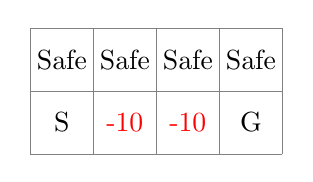
\begin{tikzpicture}[scale=0.8]
\draw[step=1cm,gray,very thin] (0,0) grid (4,2);
\node at (0.5,0.5) {S};
\node at (1.5,0.5) {\textcolor{red}{-10}};
\node at (2.5,0.5) {\textcolor{red}{-10}};
\node at (3.5,0.5) {G};
\node at (0.5,1.5) {Safe};
\node at (1.5,1.5) {Safe};
\node at (2.5,1.5) {Safe};
\node at (3.5,1.5) {Safe};
\end{tikzpicture}
\end{center}

Actions: Up, Down, Left, Right. Reward: -1 per step, -10 for cliff, +10 for goal.

\textbf{With $\epsilon$-greedy exploration:}

\textbf{Q-Learning Policy:}
\begin{itemize}
\item Learns optimal path: S → Right → Right → Right → G
\item Ignores exploration mistakes in learning
\item Takes risky path along cliff
\end{itemize}

\textbf{SARSA Policy:}
\begin{itemize}
\item Learns safe path: S → Up → Right → Right → Right → Down → G
\item Accounts for exploration mistakes
\item Takes safer path away from cliff
\end{itemize}

\textbf{Reason:} SARSA considers that random exploration might accidentally step off the cliff, so it learns a safer policy.
\end{solution}

\part When would you choose SARSA over Q-learning and vice versa?

\begin{solution}
\textbf{Choose SARSA when:}
\begin{itemize}
\item Safety is critical (autonomous vehicles, medical applications)
\item Environment has dangerous states to avoid
\item Want policy that accounts for exploration/uncertainty
\item Online learning where you care about performance during learning
\item Need conservative, risk-averse behavior
\end{itemize}

\textbf{Choose Q-Learning when:}
\begin{itemize}
\item Want to find optimal policy eventually
\item Can afford some risky exploration during learning
\item Have replay buffer or offline data
\item Environment allows recovery from mistakes
\item Need sample efficiency
\item Building on top of other algorithms (DQN, etc.)
\end{itemize}

\textbf{Summary:} SARSA for safety, Q-learning for optimality.
\end{solution}

\end{parts}

% =====================================================
% PART V: ADVANCED TD CONCEPTS
% =====================================================

\section*{Part V: Advanced TD Concepts}

\question \textbf{Bias-Variance Trade-off in TD Learning}

\begin{parts}
\part Compare the bias and variance characteristics of Monte Carlo, TD(0), and Dynamic Programming.

\begin{solution}
\begin{center}
\begin{tabular}{|p{3cm}|p{3cm}|p{3cm}|p{4cm}|}
\hline
\textbf{Method} & \textbf{Bias} & \textbf{Variance} & \textbf{Explanation} \\
\hline
Monte Carlo & Low/Zero & High & Uses true returns but high sampling variance \\
\hline
TD(0) & Medium & Medium & Bootstraps from estimates, moderate variance \\
\hline
Dynamic Programming & Zero & Zero & Uses true model, no sampling \\
\hline
\end{tabular}
\end{center}

\textbf{Key Insights:}
\begin{itemize}
\item \textbf{Bias} comes from using estimates instead of true values
\item \textbf{Variance} comes from sampling randomness
\item TD(0) provides a good middle ground between MC and DP
\end{itemize}
\end{solution}

\part Explain why TD learning often converges faster than Monte Carlo in practice.

\begin{solution}
TD learning converges faster because:

\textbf{Immediate Updates:}
\begin{itemize}
\item Updates after every step vs waiting for episode end
\item Information propagates through states immediately
\item Learns from partial episodes
\end{itemize}

\textbf{Lower Variance:}
\begin{itemize}
\item TD target has lower variance than full return
\item Less affected by random events later in episode
\item More stable learning signal
\end{itemize}

\textbf{Bootstrapping Benefits:}
\begin{itemize}
\item Uses current best estimates to improve learning
\item Information from one state helps neighboring states
\item Exploits Markov property effectively
\end{itemize}

\textbf{Example:} In a long episode, MC must wait until the end to update any values, while TD updates at each step, allowing faster propagation of value information.
\end{solution}

\end{parts}

\question \textbf{TD Learning Applications}

\begin{parts}
\part Design a TD learning approach for a robot navigation problem. Specify states, actions, rewards, and explain your choices.

\begin{solution}
\textbf{Robot Navigation Problem: Office Delivery Robot}

\textbf{States:}
$(x, y, \text{battery}, \text{carrying\_package})$
\begin{itemize}
\item $(x,y)$: Grid position in office
\item $\text{battery} \in \{1,2,3,4,5\}$: Battery level
\item $\text{carrying\_package} \in \{0,1\}$: Has package or not
\end{itemize}

\textbf{Actions:}
$\{\text{North, South, East, West, Pickup, Drop, Charge}\}$

\textbf{Rewards:}
\begin{itemize}
\item $+100$: Successfully deliver package
\item $-1$: Each time step (efficiency incentive)
\item $-50$: Battery runs out
\item $-10$: Collision with obstacle
\item $+5$: Charge at charging station
\end{itemize}

\textbf{Algorithm Choice:} Q-learning with $\epsilon$-greedy
\begin{itemize}
\item Off-policy allows learning from mistakes
\item Can learn optimal paths while exploring safely
\item No model required - learns from experience
\end{itemize}
\end{solution}

\part Discuss potential challenges and solutions when applying TD learning to this problem.

\begin{solution}
\textbf{Challenges and Solutions:}

\textbf{1. Large State Space}
\begin{itemize}
\item \textbf{Problem:} Continuous positions, many state combinations
\item \textbf{Solution:} Function approximation (neural networks), state discretization, feature engineering
\end{itemize}

\textbf{2. Safety During Exploration}
\begin{itemize}
\item \textbf{Problem:} Random actions might damage robot or environment
\item \textbf{Solution:} Safe exploration techniques, SARSA for conservative learning, simulation first
\end{itemize}

\textbf{3. Sparse Rewards}
\begin{itemize}
\item \textbf{Problem:} Only get reward at delivery - slow learning
\item \textbf{Solution:} Reward shaping, hierarchical RL, intrinsic motivation
\end{itemize}

\textbf{4. Non-Stationary Environment}
\begin{itemize}
\item \textbf{Problem:} Office layout changes, people moving around
\item \textbf{Solution:} Continuous learning, higher learning rates, recency weighting
\end{itemize}

\textbf{5. Real-Time Constraints}
\begin{itemize}
\item \textbf{Problem:} Must make decisions quickly
\item \textbf{Solution:} Efficient Q-table updates, prioritized experience replay
\end{itemize}
\end{solution}

\end{parts}

\question \textbf{Theoretical Understanding}

\begin{parts}
\part Prove that the TD error can be written as the sum of changes in value estimates along a trajectory.

\begin{solution}
\textbf{Claim:} For any trajectory, the sum of TD errors equals the difference between the actual return and initial value estimate.

\textbf{Proof:}
Consider trajectory: $s_t, s_{t+1}, \ldots, s_T$ with rewards $r_{t+1}, r_{t+2}, \ldots, r_T$.

The TD error at each step:
\begin{align}
\delta_k &= r_{k+1} + \gamma V(s_{k+1}) - V(s_k)
\end{align}

Summing from $t$ to $T-1$:
\begin{align}
\sum_{k=t}^{T-1} \delta_k &= \sum_{k=t}^{T-1} [r_{k+1} + \gamma V(s_{k+1}) - V(s_k)]\\
&= \sum_{k=t}^{T-1} r_{k+1} + \gamma \sum_{k=t}^{T-1} V(s_{k+1}) - \sum_{k=t}^{T-1} V(s_k)\\
&= G_t + \gamma V(s_T) - V(s_t)
\end{align}

Since $V(s_T) = 0$ (terminal state):
\begin{equation}
\sum_{k=t}^{T-1} \delta_k = G_t - V(s_t)
\end{equation}

This shows TD errors accumulate to the Monte Carlo error.
\end{solution}

\part Explain the relationship between TD(0), TD(1), and Monte Carlo methods.

\begin{solution}
\textbf{TD(n) Family:}

\textbf{TD(0):} Uses 1-step return
\begin{equation}
\text{Target} = r_{t+1} + \gamma V(s_{t+1})
\end{equation}

\textbf{TD(1):} Uses 2-step return
\begin{equation}
\text{Target} = r_{t+1} + \gamma r_{t+2} + \gamma^2 V(s_{t+2})
\end{equation}

\textbf{TD(n):} Uses n-step return
\begin{equation}
\text{Target} = \sum_{k=0}^{n-1} \gamma^k r_{t+k+1} + \gamma^n V(s_{t+n})
\end{equation}

\textbf{Monte Carlo (TD($\infty$)):} Uses full return
\begin{equation}
\text{Target} = G_t = \sum_{k=0}^{T-t-1} \gamma^k r_{t+k+1}
\end{equation}

\textbf{Spectrum Properties:}
\begin{itemize}
\item As $n \to 0$: More bias, less variance, faster updates
\item As $n \to \infty$: Less bias, more variance, delayed updates
\item TD($\lambda$) provides smooth interpolation between these extremes
\end{itemize}
\end{solution}

\end{parts}


\end{questions}


\end{document}
